\chapter{Dataset}
In chapter \ref{chap:give-challenge} it was mentioned, that some teams participating in GIVE Challenge tried to use a corpora of a human to human interactions in GIVE scenario. They were learning language expression or decision-making process and applying them in their NLG systems. The teams were however relying on small self-collected datasets. In a light of this, organizers of GIVE Challenge decided they would collect and provide dataset for future use. This chapter serves as an introduction and analysis of this dataset.

As a side note, \citet{striegnitz2012referring} report on a smaller German dataset, which is similar to the one I will be talking about. 

In the first section, I will introduce the dataset and provide technical details of how it was created. Second section, will, after the fashion of GIVE Challenge look how world and demographic factors influenced the task performance. Next section analyses REs in the dataset. Last section explores a phenomenon of chains of references.

\section{General overview}
The data-collection started in July and finished November of 2012. Through that period 21 interactions between two human subjects were recorded. Originally, 22 pairs participated, but one of the pair failed to finish the tasks and is excluded from the dataset. The subjects were asked to bring someone they know and they were financially compensated for the effort. 

The set-up for the experiment is in the figure \ref{fig:give-experiment-setup}. One human subject was an instruction giver (IG). He is on the right in the figure \ref{fig:give-experiment-setup}. His role was essentially the role of NLG system in GIVE Challenge. He/she was able to see a map of the world, which was updated in real-time and he/she got information about all necessary steps to finish the task. In addition, he was able to see the other's person client screen. He communicated with the other person through a microphone and his goal was to navigate the other person through the world and make him finish the treasure-hunt.

\begin{figure}[!htbp]
  \centering
	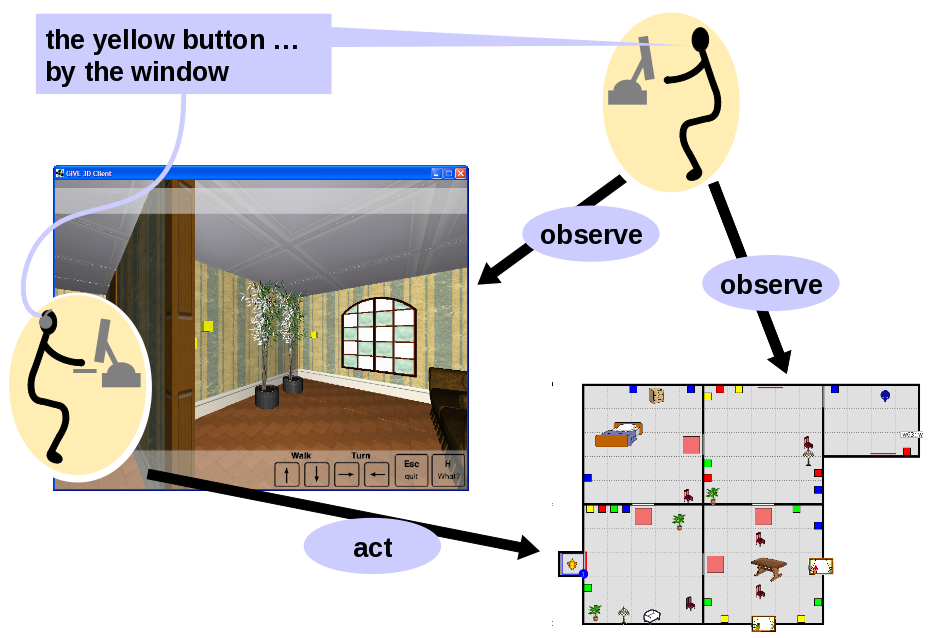
\includegraphics[width=0.7\textwidth]{Images/experiment-set-up}
	\caption{Experiment set-up of data collection}
	\label{fig:give-experiment-setup}
\end{figure}

The other person was an instruction follower (IF). He/she is on the left in the figure \ref{fig:give-experiment-setup}. He/she interacted with the client and moved the avatar around the world and was able to press buttons. IF listened to IG's instructions through a headset.

Each pair did one short tutorial world. After that they switched roles of instruction giver and instruction follower. Following was one ``normal'' world randomly chosen from two variants, marked world 1 and world 3 in the dataset. Maps of the worlds 1 and 3 are in the figures \ref{fig:dataset-world1} and \ref{fig:dataset-world3} respectively. Finally they did a difficult version of the other variant (if they started with world 1 the difficult version was for world 3 and vice versa). The difficult versions are marked 1-d and 3-d in the dataset. A difficult version of the world had an increased number of distracting buttons and landmarks compared to the ``normal'' version, as can be seen in the map of world 1-d in figure \ref{fig:dataset-world1d}. If not present in the report or not stated otherwise, the short tutorial worlds are normally excluded from the analysis.

\begin{figure}[!htbp]
  \centering
	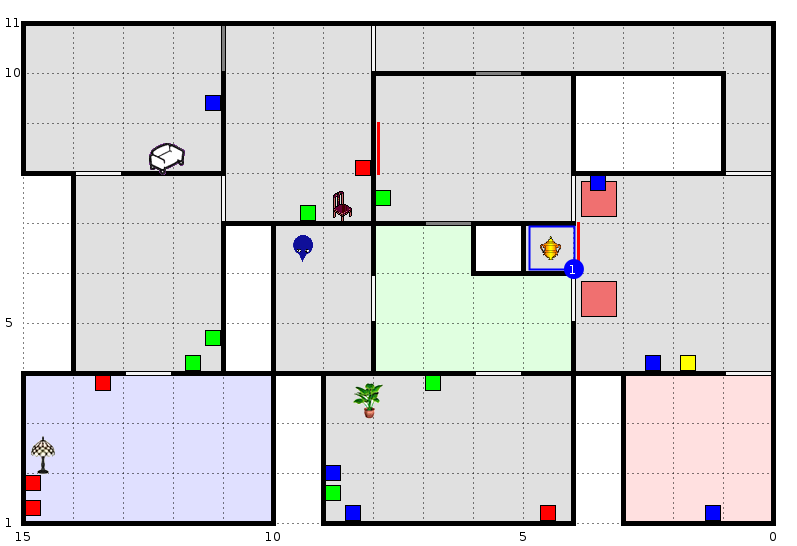
\includegraphics[width=0.7\textwidth]{Images/dataset-world1}
	\caption{Map of the world 1 - normal version.}
	\label{fig:dataset-world1}
\end{figure}

\begin{figure}[!htbp]
  \centering
	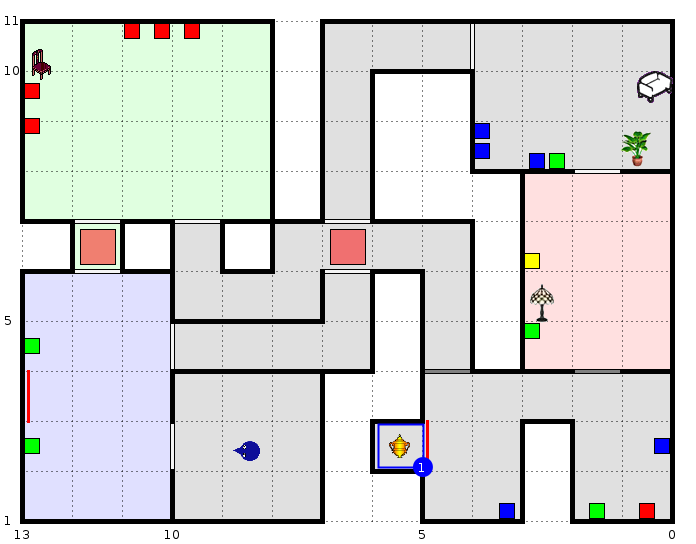
\includegraphics[width=0.7\textwidth]{Images/dataset-world3}
	\caption{Map of the world 3 - normal version.}
	\label{fig:dataset-world3}
\end{figure}

\begin{figure}[!htbp]
  \centering
	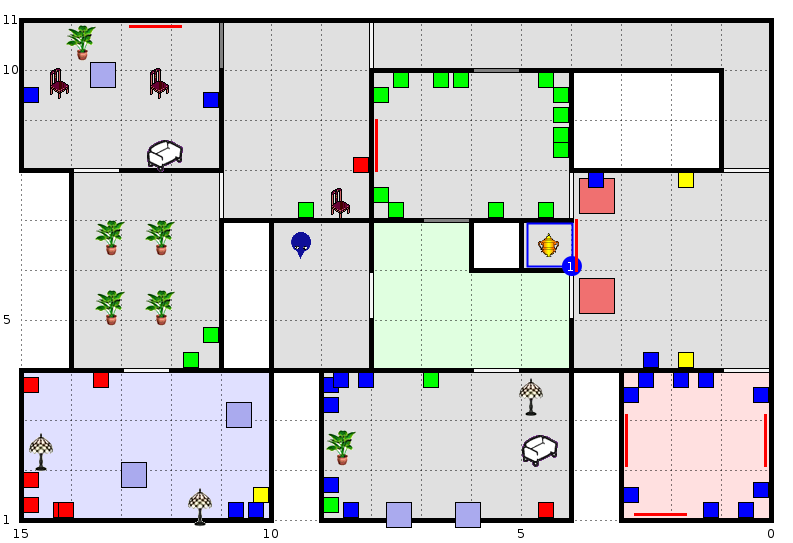
\includegraphics[width=0.7\textwidth]{Images/dataset-world1d}
	\caption{Map of the world 1 - difficult version.}
	\label{fig:dataset-world1d}
\end{figure}

Similarly to the GIVE Challenge, after all 3 rounds subjects were asked to fill a questionnaire. Its purpose was to get demographic and other relevant information on subjects. The questionnaire can be divided into three parts. First part was only filled out by IF and rated IG and his instruction giving on a scale from 1 to 7. Complete list of its questions follows: 

\begin{table}
\begin{enumerate}
\item
Overall, my partner gave me good instructions.
\item
Interacting with my partner wasn't annoying at all.
\item
My partner's instructions were clearly worded.
\item
When I had problems with the instructions, we solved them quickly.
\item
I enjoyed solving the task.
\item
I felt I could trust my partner's instructions.
\item
I really wanted to find that trophy.
\item
My partner immediately offered help when I was in trouble.
\item
I would recommend this experiment to a friend.
\item
My partner's instructions were not repetitive.
\end{enumerate}
\end{table}

Second part was filled by both IF and IG and was concerned with their navigation skills. To measure the ability to navigate in the world the Santa Barbara Sense of Direction (SBSOD) scores were used \citet{hegarty2002development}. Again the questions were on a scale from 1 to 7. Note that some of the question in the following list are of positive nature (higher rating equals better navigation skill) while other are of negative nature, therefore these scores had to be normalized.

\begin{table}
\begin{enumerate}
\item
I am very good at giving directions.
\item
I have a poor memory for where I left things.
\item
I am very good at judging distances.
\item
My "sense of direction" is very good.
I tend to think of my environment in terms of cardinal directions (N, S, E, W).
\item
I very easily get lost in a new city.
\item
I enjoy reading maps.
\item
I have trouble understanding directions.
\item
I am very good at reading maps.
\item
I don't remember routes very well while riding as a passenger in a car.
\item
I don't enjoy giving directions.
\item
It's not important to me to know where I am.
\item
I usually let someone else do the navigational planning for long trips.
\item
I can usually remember a new route after I have travelled it only once.
\item
I don't have a very good "mental map" of my environment.
\end{enumerate}
\end{table}

Finally, the last part of the questionnaire was of a demographic character. We can see questions about age, gender, language and computer expertise, 3D games experience and knowledge of the partner in following list.

\begin{table}
\begin{enumerate}
\item
What is your age?
\item
Are you male of female?
\item
What is your profession / major / favorite subject in school?
\item
How would you rate your computer expertise?
\item
How familiar are you with 3D computer games?
\item
How many hours per week to you play 3D computer games?
\item
Was there a time in your life when you played more 3D computer games? If so, how many hours did you play then?
\item
What languages do you speak? Please indicate how well you speak each on a scale from 1-5, where 5 is your native language.
\item
Did you already know the second participant?
\item
How well do you know the second participant?
\item
Have you worked collaboratively with the second participant before? (For example, when doing homework or preparing a class presentation?)
\item
Have you played 3D computer games with the second participant before?
\end{enumerate}
\end{table}

Many of these questions are explored in the next section as a potential factors influencing the task performance. 

As was mentioned in chapter \ref{chap:give-challenge}, the entire session is logged to the database. The player's position, orientation and all visible objects are logged at fixed rate. Moreover, other information as buttons presses or an end of the session are also stored in the logs. Because the worlds are static, distances and angles between player and other game's objects are easily computed from these logs.

Apart from logs, there are of course sound files of IG giving directions. These were transcribed and together with some information from the logs transformed into ELAN files. ELAN is an annotation software \citep{sloetjes2008annotation}. I will use the term automatic annotations for the ELAN files created from logs and transcribed audio. 

Building on top of these automatic annotations are manual annotations. They are primarily concerned with referring expressions and also stored in ELAN format. Most referring expressions in GIVE aim to locate a button, which needs to be pressed. I will call the button, which is a goal of an referring expression, the target button. Which button is the target button of a reference is one of the layers in the manual annotations. Another layer of the annotations is some basic grouping of the references. Whether it is a reference to a single button, to a group of button, to a landmark and so on. Third layer looks deeper into the contents of the reference. It notes whether the reference contains for example the color of a button, whether distractors or landmarks are part of the reference or whether the reference explicitly points out that the button was already pressed before.

Previously mentioned logs, automatic annotations and manual annotations together form the dataset this chapter is dealing with.

An example of what can be extracted from the data is in the following text. Spatial information are transcribed in parentheses for the sake of clearness.

\begin{verse}
(IF enters a room)\\
IG: Go towards the red buttons.\\
(IF turns right and start walking, but he turns too much)\\
IG: No the ones next to the lamp...\\
(IF corrects his direction)\\
IG: Yeah that lamp. On the right.\\
(IF is facing three buttons.)\\
IG: Press the button on the wall you are looking at, that's far from the lamp and on the left. \\
(IF goes towards the correct button and stops close to him)\\
IG: Press it.\\
\end{verse}

\section{World and Demographic factors}
As was noted repeatedly in the chapter \ref{chap:give-challenge}, the world had significant influence on the task success rate in GIVE Challenge. However the dataset was created in a different manner, so the question about influence of worlds must be reformulated. First of all, all the sessions were successful except for a one which was discarded. Therefore, the task success rate no longer makes sense. Instead, I will measure task performance by time required to finish the task (duration) and also use other performance measure when appropriate. Secondly, the normal worlds were designed to have the same or similar difficulty in order to minimize effects outside of navigation strategy. Same idea goes with the difficult worlds.

Despite the design choices, I found out that the normal worlds 1 and 3, had a different mean duration (p-value $0.0473$ for two-sample t-test). There are multiple explanation for this difference. Relatively small number of subjects is certainly one of them. We can also notice in the figure \ref{fig:dataset-world3} slightly complicated system of hallways in the center of world-3. But this discovery does not have major influence on my work. Moreover, the difficult world did not have significant difference between their mean duration (p-value $0.6195$ for two-sample t-test).

Another thing I was interested in was influence of gaming experience of both participants on certain performance measures, namely on the duration, on the average speed of IF movement and the time IF spent moving. The average speed of IF is simply a total distance the avatar controller by IF travelled in a session divided by duration. The time IF spent moving aggregates time where avatar was either motionless or only rotating in place. 

I found correlations between gaming experiences and these variables. Not surprisingly, these correlation are especially high for IF, since he/she is the one who is actually playing the world. The past gaming experience (questions 7 in third part of the questionnaire) are more important than contemporary playing (question 6 in the third part of the questionnaire). Most prominent are the hours per week spent playing of IF at the past peak gaming period (question 7), the same variable for IG and hours spent gaming per week for IF at present (question 6). For the difficult worlds some correlations change slightly. In general, individuals who are familiar with games (gamers) take less time to finish the world, they spent more time moving and they have higher speed.

The influence of SBSOD scores (second part of the questionnaire) on the task proficiency was another thing I have looked at. Correlation matrix revealed weak or almost no correlation between SBSOD scores and time needed to complete the world.

The data suggest that there is positive correlation between male gender and task proficiency measured in the duration. The effect of male IG diminishes in the difficult worlds but the effect of IF is even stronger in the difficult worlds. However there are several facts to take in consideration here. First of all, we don't have enough data to have a statistically significant conclusion. This correlation might have also been caused by having more male gamers than female gamers. Lastly, there has been research about influence of gender on spatial cognition and mental rotation; an example of more recent one is \citep{geary2000sex}. They conclude that males are more proficient in tasks requiring mental rotation. Since IG have to do mental rotation while giving direction in GIVE scenario, this might be a source of correlation. Another paper worth considering on this topic is \citep{moffat1998navigation}, which found a gender difference in time required to finish a virtual maze.

The age of IF have positive correlation with task proficiency measured in the duration and in difficult worlds this correlation is one the strongest ones: 0.6. Older IF are also moving less and are generally slower. For IG the correlations have the same direction, however they are much weaker.

Lastly I was interested how familiarity of participants with each other (questions 9-12 in the third part) influenced the task performance. The knowledge of the partner had an impact on the task efficiency. What was interesting is that, previous cooperation with the partner became much more important for the difficult worlds, while not having much impact in normal worlds. One interpretation is, of course, faster learning for pairs familiar with each others. Other one might be that in the normal worlds the referring expressions are relatively simple and does not leave much space for errors. On the other hand in the difficult worlds familiarity reduce chances of misinterpretation of complex expressions.

\section{Referring expressions}
Because REs are the main focus of my research, this section serves as an introductory analysis of REs in my dataset.

Overall, 793 REs were annotated in the manual annotations. Apart from time interval of the reference, several other facts were annotated in the manual annotations. First of all, the target button of each RE was annotated. The count of distinct target buttons is 29.  

REs were also separated into 5 high-level categories depending on what they refer to. The  overview of the categories is in the following list:

\begin{itemize}
\item
Target - Referring to the target button
\item
Group - Referring to a group of buttons, one of which is the target button
\item
Landmark object - Referring to a landmark (any object or room feature, but not a button) which will then be used to locate the target button
\item
Landmark button - Referring to a distractor button as a landmark
\item
Remove button -  Referring to a distractor button to exclude it
\end{itemize}

Percentage count of the categories is in the table \ref{tab:res-groups}. References to target button are a dominant category. Around 10\% of references are group references. References to landmarks occupy only 6\% of all references.

\begin{table}[h!]
\centering
\begin{tabular}{lr}
\toprule
Category  & Percentage (\%)  \\
\midrule
Target   		& 82.47\\
Group 			& 10.34\\
Landmark object 	& 5.04\\
Landmark button	& 1.39\\
Remove button 	& 0.76\\
\bottomrule
\end{tabular}
\caption{Percentage of REs in the groups}
\label{tab:res-groups}
\end{table} 

Manual annotations also looked into the contents of the REs.

\section{Chains of references}
Interesting phenomenon I have noticed and further explored in the dataset are consecutive references to one button. It can be seen in following sentences: ``Straight ahead of you there on the opposite wall there are two blue buttons. Press the one on the right. The one close to the picture.'' The IG started of with a references to a group of two buttons; the target button being one of those two. In the second sentence he picked out the target button from the group. In the last sentence IG made another reference containing landmark, adding redundant information. Since the references are concerned with one target button and follow each other relatively fast, I have called them chains of references (chains, in short).

The chains vary in length, from short ones, consisting of only two references, up to lengthy ones with eight references following each other. The example from previous paragraph is three references long. Figure \ref{fig:chains_len_histo} shows histogram of the chains length.

\begin{figure}[!htbp]
  \centering
	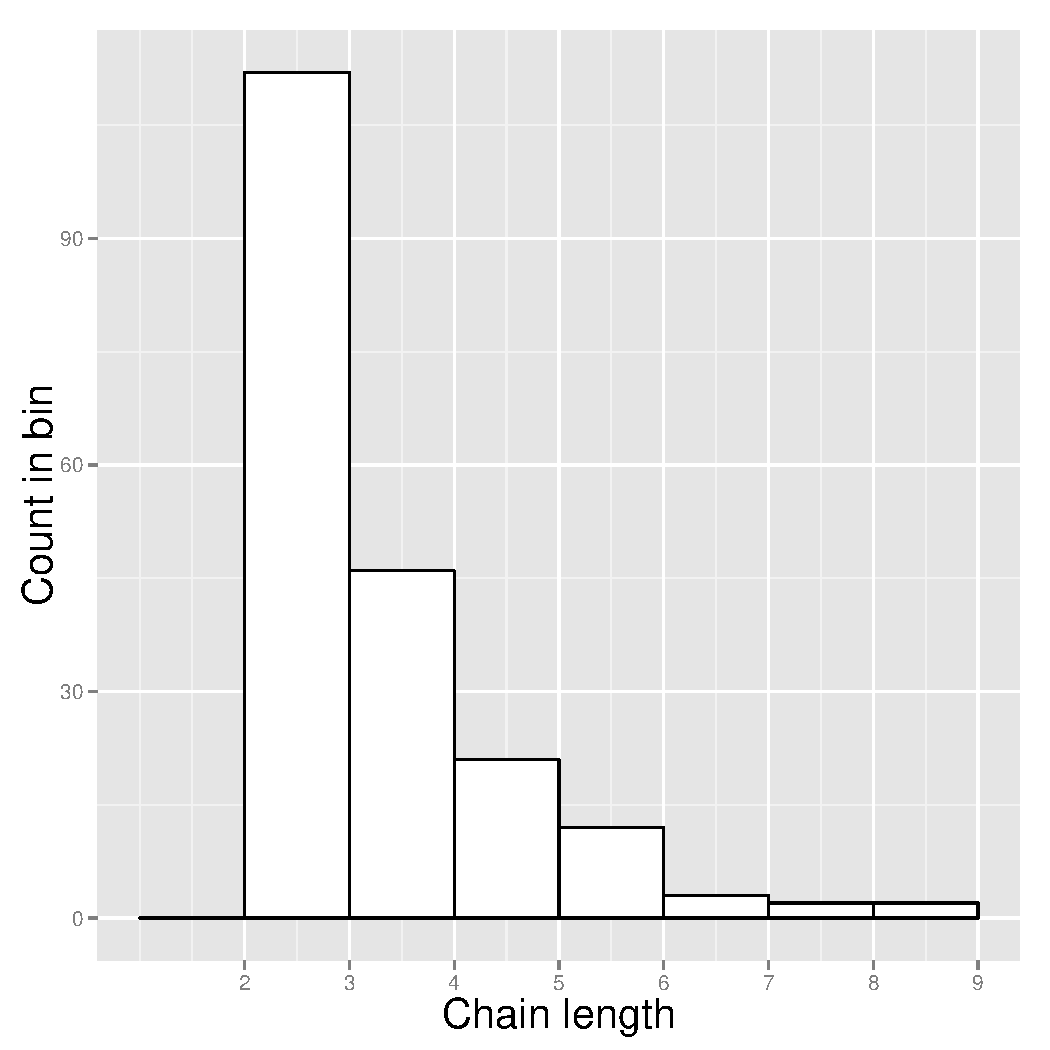
\includegraphics[width=0.8\textwidth]{Images/chains_len_histo}
	\caption{Histogram of the chain length}
	\label{fig:chains_len_histo}
\end{figure}


The chains are significant part of the discourse, in fact over 77\% of all RE belong to a chain. However, the chains have multiple linguistic functions, which makes them difficult to explore. Even inside one chain, there are often combination of functions. I have manually annotated some common functions of the chains. Most common one is to inform IF that he is supposed to press the target button. A simple example of this function, which I call action, is in following discourse: ``The red button in front of you. Press that one.'' It may sound redundant to use action function as the experiment progresses, since the IF are not manipulating the buttons in any other way than pressing them. But I have found out that it's often the case.

Another common function is confirmation: ``That same red button we pressed before, we'll press that again. Yeah that one.'' The IG confirms at the end of previous utterance that IF is looking at or heading to a correct target button.

IG often utter a RE, which does not perfectly ``picks out'' the target button from the set of buttons in the room. IG can make up for that information deficit with confirmation function or further specify with another RE. That is a specification function, as in following two sentences: ``Now that green button. You want the one closer to the lamp.''

When a group of buttons is utilized in RE and the target button is part of that group, it is inevitable that IG will have to make another RE to ``pick out'' the target button from the group. Therefore group references imply chains of references and should be considered as one of the functions. Simple example of the group function: ``Two blue buttons on the wall. Hit the blue button on the right side.''

When IF has clearly chosen the wrong button, IG will try to correct that error. I call that an error function. Following extract features this function: ``That blue button. No no no. The other. That one.''

Summary of the functions is in the table \ref{tab:chains-functions}. Please note that these functions are not exclusive. One chain can have both confirmation and specification function.

\begin{table}[h!]
\centering
\begin{tabular}{lr}
\toprule
Function   & Chains containing it (\%)  \\
\midrule
Action    		& 66.16\\
Confirmation	 	& 29.29\\
Specification 	& 25.25\\
Group 	  		& 24.74\\
Error 			& 11.11\\
\bottomrule
\end{tabular}
\caption{Percentage of chains having specific functions}
\label{tab:chains-functions}
\end{table}



